%!TEX root = volumeFinal.tex 
\chapter{\label{chap:agentes}Agentes} 

\frm[inline]{De repente reestruturar um pouco esta seção para falar de agentes e jogos e começar com uma motivação mais complexa ao invés de só dropar a frase dos agentes nos jogos...}

Os agentes são utilizados em jogos como uma abstração que represente os jogadores. Os agentes conseguem absorver informações providas do jogo e assim decidir qual o próximo passo a ser tomado \cite{millington2009artificial}. 

Formalmente, agentes são entidades que agem de forma continua e autônoma em um ambiente \cite{agent1993oriented}. 
Os agentes são capazes de receber estímulos do ambiente através de sensores, e assim responder aos estímulos por intermédio de atuadores. 
Para os agentes os estímulos do ambiente são recebidos como percepções. 
Os atuadores por sua vez, geram, uma ação considerando as percepções \cite{intelligence2003modern}. 
A interação de um agente com o ambiente pode ser ilustrado pela Figura~\ref{fig:agente}.

\begin{figure}[ht]
	\centering
	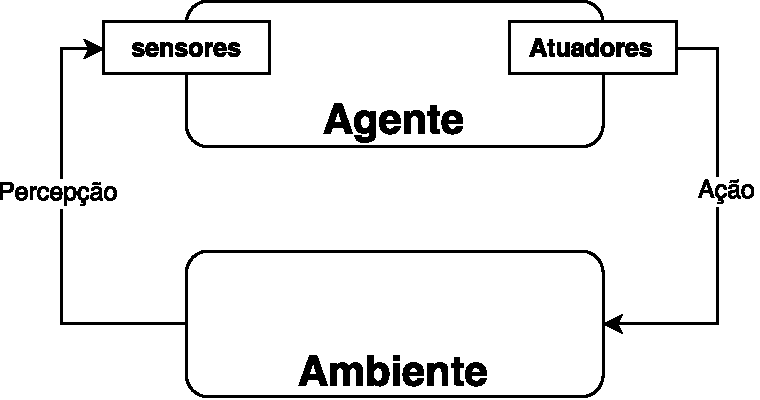
\includegraphics[width=0.5\textwidth]{fig/agente.pdf}
	\caption{Representação de um agente}
	\label{fig:agente}
\end{figure} 

O agente deve agir de forma autônoma, para isso ele deve ser capaz de aprender a lidar com situações proporcionadas pelo ambiente, com o intuito de realizar ações em busca do seu objetivo. O agente precisa de três características para conseguir ser autônomo \cite{agent1999}. São elas:
 
\begin{itemize}
	\item reatividade, para que os agentes sejam capazes de perceber o ambiente e suas mudanças a fim de levar o ambiente em consideração para a tomada de decisão das ações;
	\item pró-atividade, para que os agentes consigam ter a iniciativa em tomar as suas ações; e
	\item habilidade social, para que os agentes sejam capazes de interagir com outros agentes(humanos ou não).
\end{itemize}

As duas primeiras características são necessárias para que o agente consiga interagir com o ambiente. Um agente sendo reativo, ele consegue, a partir de uma mudança do ambiente, saber como ele deve se comportar. Sendo proativo, o agente pode antecipar suas ações em busca do seu objetivo.
Nem sempre um agente vai estar sozinho no ambiente, por esse motivo, a terceira característica é necessária para que o agente consiga interagir com outros agentes. Sistemas onde existem mais de um agente são chamados de sistema multi agentes. Nesses sistemas, os agentes interagem entre si, podendo ter objetivos em comum ou não. Sendo assim eles terão que cooperar ou negociar entre si \cite{intelligence2003modern}.

\section{Ambientes}

O agente deve se comunicar com um ambiente para conseguir alcançar seus objetivos. Mas um ambiente é composto por diversas propriedades que podem influenciar como o agente vai agir para chegar ao seu objetivo \cite{intelligence2003modern}. 

Nem sempre todas as informações do ambiente estarão disponíveis, por esse motivo o ambiente pode ser dito como completamente observável, parcialmente observável ou não observável, dependendo da informação disponibilizada. Um ambiente é dito completamente observável se, em qualquer instante de tempo, todas as informações relevantes do ambiente estão disponíveis para os sensores do agente. Caso haja alguma informação que não possa ser acessada, em algum instante de tempo, seja por causa da incapacidade do sensor do agente de captar essas informações ou pelo fato da informação simplesmente não ser disponibilizada, o ambiente é dito parcialmente observável. Agora, se o ambiente não disponibiliza nenhuma informação, o ambiente é tido como não observável \cite{ intelligence2003modern, agent1999}.   

O ambiente pode sofrer modificações, as modificações podem ser provenientes de ações realizadas pelos agentes, ou ainda por mudanças ocasionadas pelo próprio ambiente. O ambiente é determinístico se o estado gerado após a execução de uma ação, em todas as vezes que for executada, levar para o mesmo estado resultante, ou seja, o estado resultante é determinado pelo estado atual e a ação executada pelo agente. Se não há a certeza do estado resultante, o ambiente é estocástico. Quando o ambiente é não determinístico existem chances das ações dos agentes nem lembre levarem para os estados conhecidos \cite{intelligence2003modern}. 

Os estados do ambiente irão mudar ao longo do tempo, seja por uma ação feita por algum agente, ou por alguma mudança que possa ocorrer em razão de outro processo do ambiente. Se o ambiente sofre alguma alteração apenas quando o agente executa alguma ação, o ambiente é estático. Se o ambiente tem a capacidade de mudar independente de uma ação de um agente, o ambiente é dinâmico \cite{agent1999}.

Em sistemas multi agentes os agentes podem estar competindo ou cooperando entre si. O ambiente é competitivo quando os agentes estão competindo, como em um jogo de xadrez, por exemplo, ou o ambiente é cooperativo quando os agentes estão cooperando \cite{intelligence2003modern}.

\section{Arquiteturas de Agentes}


O tipo mais simples de agente é aquele que apenas reage a uma percepção vinda do ambiente. O agente escolhe suas ações baseado no que percebe no momento da decisão, sem levar em consideração ações já tomadas ou percepções anteriores. O agente apenas responde a uma percepção com uma ação, como se houvesse um clausula condicional que determinasse qual a ação a ser tomada se acontecer alguma coisa, como por exemplo, se estiver chovendo eu irei levar um guarda-chuva. A Figura~\ref{fig:agenteSimple} ilustra essa arquitetura. 

\begin{figure}[ht]
	\centering
	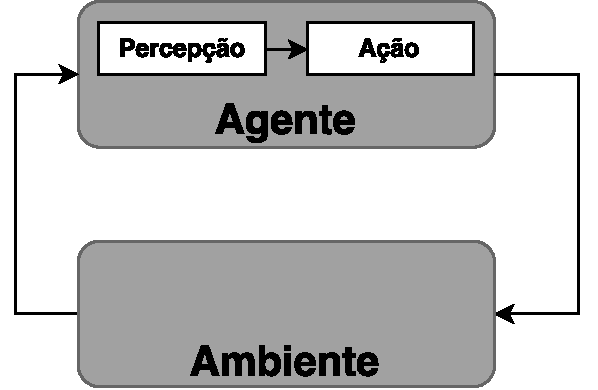
\includegraphics[width=0.4\textwidth]{fig/agentSimple.pdf}
	\caption{Arquitetura simples de um agente.}
	\label{fig:agenteSimple}
\end{figure} 


Este tipo de agente consegue ser simples, no entendimento e na sua utilização, mas a sua inteligência é limitada. Essa arquitetura é eficaz em ambientes completamente observáveis, pelo fato de que o agente precisa da percepção para realizar a sua ação \cite{intelligence2003modern}. A arquitetura pode ser usada, por exemplo, quando for preciso conhecer um conjunto de cidades, o agente após chegar a uma cidade, vai para a próxima cidade ao norte da cidade atual, quando não há norte ele vai para oeste. 

Na tentativa de aprimorar as decisões tomadas pelo agente, pode-se usar um estado interno para marcar qual a situação do ambiente. A informação representada no estado pode ser alguma informação que não consiga ser obtida por alguma percepção do ambiente ou de estados que já foram visitados pelo agente, por exemplo \cite{intelligence2003modern}. A Figura~\ref{fig:agenteModelbased} ilustra esta arquitetura. 

\begin{figure}[ht]
	\centering
	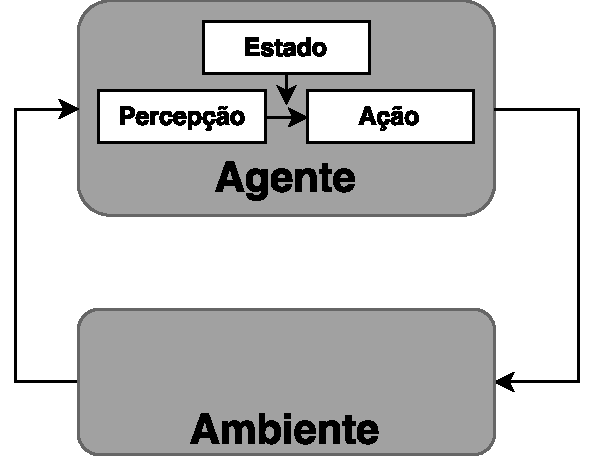
\includegraphics[width=0.4\textwidth]{fig/agentModel.pdf}
	\caption{Arquitetura de agentes com estados.}
	\label{fig:agenteModelbased}
\end{figure} 

Este tipo de arquitetura é eficaz para ambientes parcialmente observáveis, pelo fato de que o estado pode guardar informações relevantes para o agente \cite{intelligence2003modern}. No exemplo de conhecer as cidades, se guardar as visitas antigas, pode ajudar a não visitar novamente cidades que já tiverem sido visitadas. 

Dependendo do intuito do agente, conhecer o estado atual do ambiente não é suficiente. Além de estado, o agente pode precisar de uma informação para saber onde ele quer chegar, ou seja, um objetivo. Um objetivo é usado para descrever o que o agente está almejando alcançar. Para o agente conseguir alcançar o objetivo com uma melhor performance pode ser utilizado uma função de utilidade, nesta função é medido o "desejo" do agente em tomar determinada ação. Cada ação exercida pelo agente terá influência no valor de utilidade obtido \cite{intelligence2003modern}. Seguindo no exemplo, o objetivo pode ser visitar todas as cidades e a função de utilidade pode medir a distância entre as cidades, e assim podendo alcançar o objetivo com a menor distância percorrida. 


